\documentclass[tikz,border=10pt]{standalone}
\usepackage{tikz}
\usetikzlibrary{shapes.geometric,arrows.meta,positioning,fit,backgrounds,calc}

\begin{document}
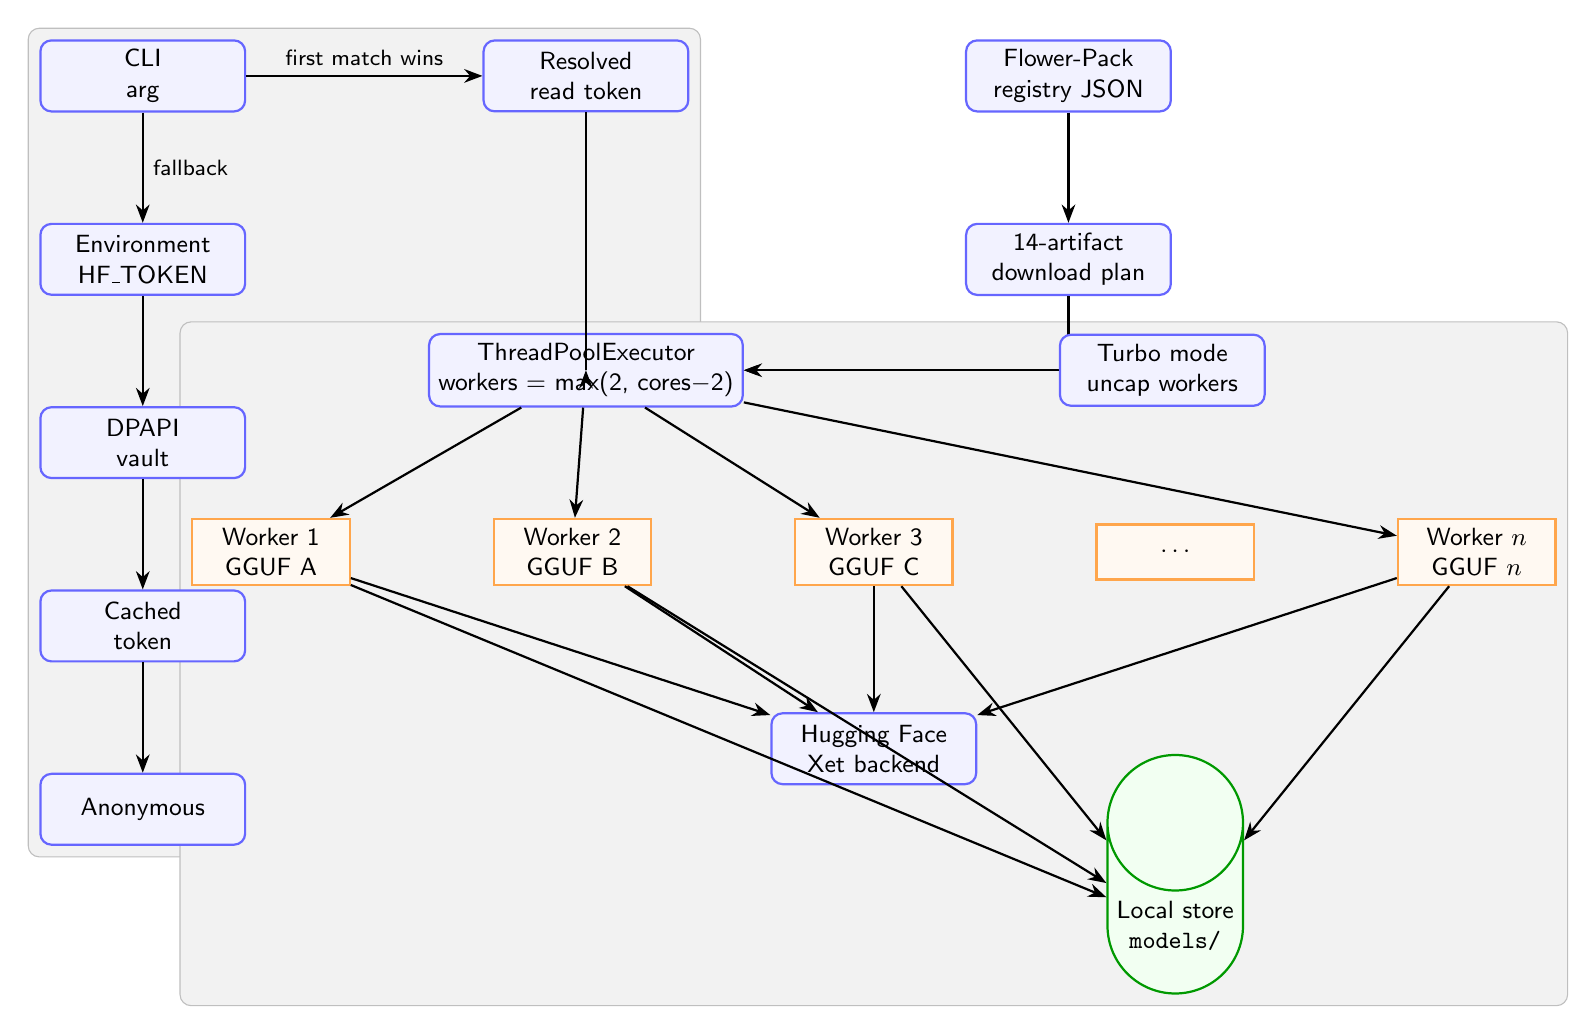
\begin{tikzpicture}[
	font=\sffamily\small,
	node distance=1.4cm and 1.8cm,
	>=Stealth,
	box/.style={rectangle, rounded corners, draw=blue!60, fill=blue!5, minimum width=2.6cm, minimum height=0.9cm, align=center, thick},
	worker/.style={rectangle, draw=orange!70, fill=orange!5, minimum width=2cm, minimum height=0.7cm, align=center, thick},
	store/.style={cylinder, shape border rotate=90, draw=green!60!black, fill=green!5, minimum width=1.6cm, minimum height=0.8cm, align=center, thick},
	label/.style={rectangle, draw=gray!50, fill=gray!10, rounded corners, inner sep=4pt, font=\bfseries\small}
]

% --- Token resolution chain ---
\node[box] (cli) {CLI\\arg};
\node[box, below=of cli] (env) {Environment\\HF\_TOKEN};
\node[box, below=of env] (vault) {DPAPI\\vault};
\node[box, below=of vault] (cached) {Cached\\token};
\node[box, below=of cached] (anon) {Anonymous};

\draw[->, thick] (cli) -- (env) node[midway,right]{\footnotesize fallback};
\draw[->, thick] (env) -- (vault);
\draw[->, thick] (vault) -- (cached);
\draw[->, thick] (cached) -- (anon);

\node[box, right=3cm of cli] (resolved) {Resolved\\read token};
\draw[->, thick] (cli) -- (resolved) node[midway,above]{\footnotesize first match wins};

% --- Registry plan ---
\node[box, right=3.5cm of resolved] (reg) {Flower-Pack\\registry JSON};
\node[box, below=of reg] (plan) {14-artifact\\download plan};
\draw[->, thick] (reg) -- (plan);

% --- Pool ---
\node[box, below=2.8cm of resolved] (pool) {ThreadPoolExecutor\\workers = max(2, cores$-$2)};
\draw[->, thick] (resolved) |- (pool);
\draw[->, thick] (plan) |- (pool);

% --- Workers ---
\node[worker, below=of pool, xshift=-4cm] (w1) {Worker 1\\GGUF A};
\node[worker, right=of w1] (w2) {Worker 2\\GGUF B};
\node[worker, right=of w2] (w3) {Worker 3\\GGUF C};
\node[worker, right=of w3] (wdots) {$\cdots$};
\node[worker, right=of wdots] (wn) {Worker $n$\\GGUF $n$};

\draw[->, thick] (pool) -- (w1);
\draw[->, thick] (pool) -- (w2);
\draw[->, thick] (pool) -- (w3);
\draw[->, thick] (pool) -- (wn);

% --- Backend / network ---
\node[box, below=1.6cm of w3] (hf) {Hugging Face\\Xet backend};
\node[store, below=2.2cm of wdots] (store) {Local store\\\texttt{models/}};

\foreach \w in {w1,w2,w3,wn} {
  \draw[->, thick] (\w) -- (hf);
  \draw[->, thick] (\w) -- (store);
}

% --- Turbo mode ---
\node[box, right=4cm of pool] (turbo) {Turbo mode\\uncap workers};
\draw[->, dashed] (turbo) -- (pool);

\begin{scope}[on background layer]
  \node[fit=(cli)(anon)(resolved),fill=blue!3,rounded corners,inner sep=10pt,label={[label]above left:Token resolution}]{\hspace{1cm}};
  \node[fit=(pool)(w1)(wn)(store),fill=orange!3,rounded corners,inner sep=10pt,label={[label]above right:Concurrent download}]{\hspace{1cm}};
\end{scope}

\end{tikzpicture}
\end{document}
